%%%%%%%%%%%%%%%%%%%%%%%%%%%%%%%%%%%%%%%%%%%%%%
% Header
\documentclass[11pt]{report}
\usepackage[english]{babel}
\usepackage[utf8x]{inputenc}
\PassOptionsToPackage{hyphens}{url}\usepackage{hyperref}
\usepackage{graphicx}
\usepackage{fullpage}
\usepackage{nicefrac}
\usepackage[lastexercise]{exercise}
\usepackage[dvipsnames]{xcolor}
\usepackage{listings}
\usepackage{enumitem}
\graphicspath{ {./img/} }

\setlength{\parindent}{0cm}

\renewcommand{\ExerciseHeader}{\large\textbf{\ExerciseName~\ExerciseHeaderNB} - \textbf{\ExerciseTitle}\medskip}

\renewcommand{\ExePartHeader}{\medskip\textbf{\ExePartName\ExePartHeaderNB\ExePartHeaderTitle\medskip}}

\begin{document}
%%%%%%%%%%%%%%%%%%%%%%%%%%%%%%%%%%%%%%%%%%%%%%
\title{Exercises -- Week 9: New Title}
\subsubsection*{EMAT10007 -- Introduction to Computer Programming}
\section*{\Large Exercises -- Week 10. Matplotlib}

\subsection*{\Large 10.1 Plotting}

\textbf{Note:} A widely-used way to import the matplotlib module is by adding the following line at the start of your code: {\tt import matplotlib.pyplot as plt}. Any function belonging to the  matplotlib module can then be accessed by writing, for example, {\tt plt.plot()}.

All data used in these exercises can be found in the {\tt sample\_data} folder which can be downloaded as a zip file from blackboard. 


\begin{Exercise}[title= Line and scatter graphs (Essential)] 
\label{Ex:Variables}
	\Question{Create two lists of integers named {\tt x} and {\tt y} with the following values: \\
	{\tt x = [0,2,4,5,8,10,13]}\\
	{\tt y = [1,3,3,3,4,5,6]}\\
	Generate a scatter plot of {\tt y} against  {\tt x} .}\\
	\textbf {Hint:}	Remember to use {\tt plt.show()} to display the graph.
	\Question{Modify the format string to change the appearance of the graph.}

	\Question{On the same axes, plot the graph of {\tt f} against  {\tt x} and modify the format string to change the appearance of the graph.\\
	{\tt f = [-3,0,1,0,4,6,7]}}
	
% 	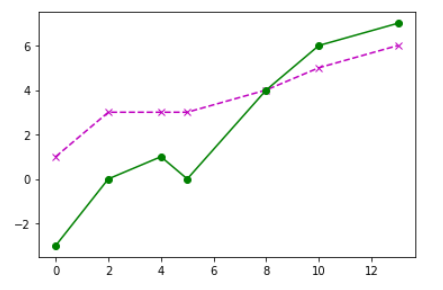
\includegraphics[height=5.5cm]{linesGraph}
%     \label{fig:linesGraph}
    
	\Question{Alter your graph so it has the following} 
	\begin{itemize}
	    \item title: {\tt Plot of y,f vs x}
	    \item x axis label: {\tt x}
	    \item legend indicating which line is {\tt y} data and which is {\tt f}
	  \end{itemize}
	  
	\Question{Save your plot as a .pdf file}

\end{Exercise}




%\newpage

\begin{Exercise}[title= Importing data (Essential)] \label{Ex:Importing_data}


\Question{Import the data from {\tt hourly\_cycle\_count\_weekend.csv} and plot a line graph of the data with `Time' on the horizontal axis and `Total' on the vertical axis. Label the axes.}

\Question{Import the data in file signal\_data.csv. Plot the data as a scatter graph where the first row is the x (horizontal) data and the second row is the y (vertical) data.}\label{Q:signal}

\Question{Import the data from {\tt temperature\_data.txt} and plot the data with the months on the horizontal axis and the temperature on the vertical axis for each city, as three scatter plots on the same graph. Add a figure legend to show which data set is which and label the axes.}\label{Q:temperature}

\end{Exercise}


\begin{Exercise}[title= Importing data for Modelling (Essential)] \label{Ex:Importing_data_modelling}

Real data is often not in the exact form we want to plot it and some data processing is required before using the data.

\Question{The file `douglas\_data.csv` contains a data set of recorded parameters for a sample of wooden beams. Convert the Bend strength to units of Nm$^{-2}$ and produce a scatter plot of bend strength against knot ratio. Label the axes.}\label{Q:beams}

\Question{The file `FremontBridge.csv` contains a data set of traffic crossing a bridge at different times of day. Produce a time series scatter plot of the data in the column `Fremont Bridge Total', for the first 2 days (the first 48 samples).}

\end{Exercise}


\begin{Exercise}[title= Importing data (Advanced)] \label{Ex:Variables}

\Question{The file FremontBridge.csv contains a data set of traffic crossing a bridge at different times of day. Produce a time series scatter plot of the data in the column 'Fremont Bridge Total', for all data, using only the sample taken at 9am for each day.}

\Question{ column `Fremont Bridge Total', for all data, bu instead use the average value taken for each day.}

\end{Exercise}


\subsection*{\Large 10.2 Curve Fitting and Exporting Data}

\begin{Exercise}[title= Curve Fitting (Essential)]\label{Ex:Curve_fitting} 

\Question{Fit a function of your choice to the scatter plot you generated in your answer to Ex \ref{Ex:Importing_data}.\ref{Q:signal} and show the fitted curve as a line on the graph. Save the plot as a .png file.}\label{Q:signal_fitting}

\Question{Fit a polynomial curve of degree 2 to each of the scatter plots in your answer to Ex \ref{Ex:Importing_data}.\ref{Q:temperature} and show each fitted curve as a line on the graph. Save the plot as a .pdf file.}\label{Q:temperature_fitting}


\end{Exercise}


\begin{Exercise}[title=Exporting data (Essential)] \label{Ex:Variables}

\Question{Export the horizontal data and the raw and fitted vertical data for each city in your answer to Ex  \ref{Ex:Curve_fitting}.\ref{Q:signal_fitting} to a .txt file.}

\Question{Export the horizontal data and the raw and fitted vertical data in your answer to Ex\ref{Ex:Curve_fitting}.\ref{Q:temperature_fitting} to a .csv file.}
\end{Exercise}


\begin{Exercise}[title= Curve Fitting for Modelling (Essential)]\label{Ex:Curve_fitting} 

\Question{Fit 3 polynomial curves of degree 1, 2 and 3 the scatter plots in your answer to Ex \ref{Ex:Importing_data_modelling}.\ref{Q:beams} and show each fitted curve as a line on the graph.}

\Question{Use a figure legend to show the degree of each fitted polynomial curve.}

\Question{Find the RMSE of each fitted curve with the raw data.}

\Question{Print the equation of the polynomial that gives the best fit.}

\Question{Save the plot as a .pdf file.}

\end{Exercise}

\begin{Exercise}[title= More Curve Fitting for Modelling (Essential)]\label{Ex:Curve_fitting}

\Question{Use the fitted data in your answer to  Ex\ref{Ex:Curve_fitting}.\ref{Q:temperature_fitting} to a .csv file. to predict the temperature in London for the months missing from the original data set. 
\\
Hint: Generate  the fitted function for all 12 months. }

\end{Exercise}









\end{document}